STEPSS is an open-source software in the sense explained in Section~\ref{sec-codegen}. Nevertheless, two power system components have their model hard-coded in the software: the synchronous machine and the Th\'{e}venin equivalent. The reason is that those components are used to define the phase angle references, as explained in Section~\ref{sec-refframe}; it would be impractical to leave this task to a user-defined model.

The constant impedance (or admittance) load is also hard-coded, since it is used at initialisation to automatically replace missing bus power injection, as explained in Section~\ref{sec-ini-proc}.

This chapter is devoted to presenting the models of those three basic components.

%------------------------------------------------------------------------------------------
\section{\index{FNOM}Nominal system frequency}

The nominal system frequency is specified by an FNOM record as follows.

\hspace*{5ex}{\tt FNOM F ;}

where {\tt F} is the value of the nominal frequency, in Hz.

Note that the presence of this record is {\bf mandatory}.

%------------------------------------------------------------------------------------------
\section{Synchronous machines}

The synchronous machine has a detailed sixth-order model, including four rotor windings with saturation effects. Models with less rotor windings can be specified by skipping some data. The notation used for the windings is shown in Fig.~\ref{fig-sync-park}.

To encompass the various combinations in a single model, ``switches'' are used. These are integer parameters defined as follows:
\begin{itemize}
\item[$S_{d1}$] = 1 if there is a damper winding $d1$, = 0 otherwise
\item[$S_{q1}$] = 1 if there is a damper winding $q1$, = 0 otherwise
\item[$S_{q2}$] = 1 if there is an equivalent winding $q2$, = 0 otherwise
\end{itemize}

The allowed combinations of $S_{d1}$, $S_{q1}$ and $S_{q2}$ are shown in the Table~\ref{tab-sync-variants}, with the corresponding values of the switches. Note that the second and third combinations yield the same results.

\begin{table}[htb]
\centering
\caption{Variants of the synchronous machine model}\label{tab-sync-variants}
\begin{tabular}{|c|c|}
\hline
model & switches \\ \hline
detailed, round rotor & $S_{d1} = 1$, $S_{q1} = 1$, $S_{q2} = 1$ \\
detailed, salient-pole rotor & $S_{d1} = 1$, $S_{q1} = 1$, $S_{q2} = 0$ \\
detailed, salient-pole rotor & $S_{d1} = 1$, $S_{q1} = 0$, $S_{q2} = 1$ \\
simplified, field winding only & $S_{d1} = 0$, $S_{q1} = 0$, $S_{q2} = 0$ \\ \hline
\end{tabular}
\end{table}

\subsection{Park transformation}

The well-known Park transformation is used to replace time-varying inductances and oscillatory stator currents and voltages with constant values. The equivalent windings are defined in Fig.~\ref{fig-sync-park}.

\begin{figure}[htb]
\centering
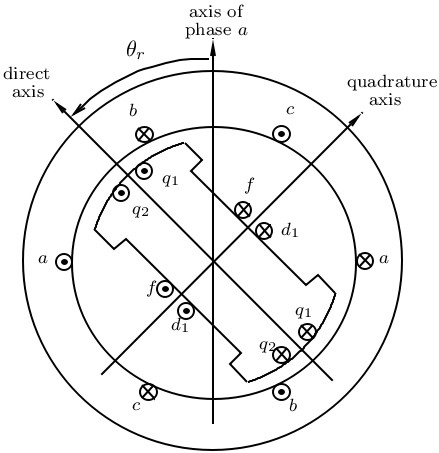
\includegraphics[width=69mm]{sync-windings.jpg}~~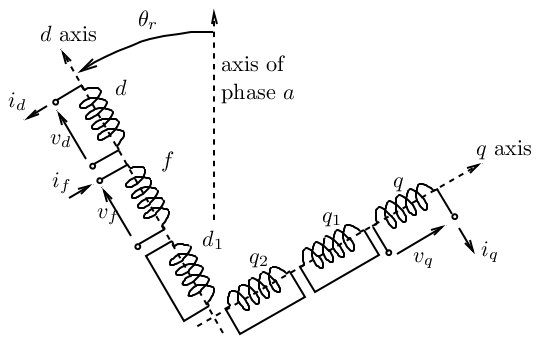
\includegraphics[width=76mm]{sync-park.jpg}
\caption{Equivalent windings of Park transformation}\label{fig-sync-park}
\end{figure}

\subsection{Flux-current relationships}

Using the Equal-Mutual-Flux-Linkage (EMFL) per unit system, the relationship between magnetic flux linkages (denoted with $\psi$) and currents (denoted with $i$) can be written as:
\begin{eqnarray}
\left[ \begin{array}{c} \psi_d \\ \psi_f \\ \psi_{d1} \end{array} \right] & = &
\left[ \begin{array}{ccc} L_\ell + M_d & M_d & S_{d1} M_d \\
M_d & L_{\ell f} + M_d & S_{d1} M_d \\
S_{d1} M_d & S_{d1} M_d & L_{\ell d1} + S_{d1} M_d \end{array} \right]
\left[ \begin{array}{c} i_d \\ i_f \\ i_{d1} \end{array} \right] \label{sync-flux-d} \\
\left[ \begin{array}{c} \psi_q \\ \psi_{q1} \\ \psi_{q2} \end{array} \right] & = &
\left[ \begin{array}{ccc} L_\ell + M_q & S_{q1} M_q & S_{q2} M_q \\
S_{q1} M_q & L_{\ell q1} + S_{q1} M_q & S_{q2} M_q \\
S_{q2} M_q & S_{q2} M_q & L_{\ell q2} + S_{q2} M_q \end{array} \right]
\left[ \begin{array}{c} i_q \\ i_{q1} \\ i_{q2} \end{array} \right] \label{sync-flux-q}
\end{eqnarray}
where $L_\ell$ is the stator leakage inductance, $L_{\ell f}$ the field winding leakage inductance, $L_{\ell d1}$, $L_{\ell q1}$, $L_{\ell q2}$ the rotor winding leakage inductances, and $M_d$ (resp. $M_q$) the direct-axis (resp. quadrature-axis) mutual inductance.

The $d$ and $q$ components of the air-gap flux are given by:
\begin{eqnarray}
\psi_{ad} & = & M_d ( i_d + i_f + S_{d1} i_{d1} ) \label{psiad-def} \\
\psi_{aq} & = & M_q ( i_q + S_{q1} i_{q1} + S_{q2} i_{q2} ) \label{psiaq-def}
\end{eqnarray}

Substituting in Eqs.~(\ref{sync-flux-d}) and (\ref{sync-flux-q}), one easily obtains:
\begin{eqnarray}
\psi_d & = & L_\ell i_d + \psi_{ad} \label{psid-airgap} \\
\psi_f & = & L_{\ell f} i_f + \psi_{ad} \label{psif-airgap} \\
\psi_{d1} & = & L_{\ell d1} i_{d1} + S_{d1} \psi_{ad} \label{psid1-airgap} \\
\psi_q & = & L_\ell i_q + \psi_{aq} \label{psiq-airgap} \\
\psi_{q1} & = & L_{\ell q1} i_{q1} + S_{q1} \psi_{aq} \label{psiq1-airgap} \\
\psi_{q2} & = & L_{\ell q2} i_{q2} + S_{q2} \psi_{aq} \label{psiq2-airgap}
\end{eqnarray}

Using Eqs.~(\ref{psif-airgap}, \ref{psid1-airgap}, \ref{psiq1-airgap}, \ref{psiq2-airgap}), the rotor currents are obtained from the flux linkages as:
\begin{eqnarray}
i_f & = & \frac{\psi_f - \psi_{ad}}{L_{\ell f}} \label{if-rotor} \\
i_{d1} & = & \frac{\psi_{d1} - S_{d1} \psi_{ad}}{L_{\ell d1}} \label{id1-rotor} \\
i_{q1} & = & \frac{\psi_{q1} - S_{q1} \psi_{aq}}{L_{\ell q1}} \label{iq1-rotor} \\
i_{q2} & = & \frac{\psi_{q2} - S_{q2} \psi_{aq}}{L_{\ell q2}} \label{iq2-rotor}
\end{eqnarray}

\subsection{Saturation model}

Let $M_d^u$ and $M_q^u$ be the {\em unsaturated} direct- and quadrature-axis mutual inductances, related to their corresponding saturated values $M_d$ and $M_q$ by:
\begin{eqnarray}
M_d & = & \frac{M_d^u}{1 + m \left( \sqrt{\psi_{ad}^2 + \psi_{aq}^2} \right)^n} \label{md-sat} \\
M_q & = & \frac{M_q^u}{1 + m \left( \sqrt{\psi_{ad}^2 + \psi_{aq}^2} \right)^n} \label{mq-sat}
\end{eqnarray}

Replacing $M_d$ by the above expression and $i_f$ and $i_{d1}$ by Eqs.~(\ref{if-rotor}, \ref{id1-rotor}), respectively, the expression (\ref{psiad-def}) of the $d$-axis air-gap flux becomes:
\[
\psi_{ad} \; = \; \frac{M_d^u}{1 + m \left( \sqrt{\psi_{ad}^2 + \psi_{aq}^2} \right)^n} ( i_d + \frac{\psi_f - \psi_{ad}}{L_{\ell f}} + S_{d1} \frac{\psi_{d1} - S_{d1} \psi_{ad}}{L_{\ell d1}} )
\]

Rearranging terms yields the algebraic equation:
\begin{equation}\label{psiad-alg}
\psi_{ad} \left( \frac{1 + m \left( \sqrt{\psi_{ad}^2 + \psi_{aq}^2} \right)^n}{M_d^u} + \frac{1}{L_{\ell f}} + \frac{S_{d1}}{L_{\ell d1}} \right) - i_d - \frac{1}{L_{\ell f}} \psi_f - \frac{S_{d1}}{L_{\ell d1}} \psi_{d1} = 0
\end{equation}

Similar operations in the $q$ axis yield:
\begin{equation}\label{psiaq-alg}
\psi_{aq} \left( \frac{1 + m \left( \sqrt{\psi_{ad}^2 + \psi_{aq}^2} \right)^n}{M_q^u} + \frac{S_{q1}}{L_{\ell q1}} + \frac{S_{q2}}{L_{\ell q2}} \right) - i_q - \frac{S_{q1}}{L_{\ell q1}} \psi_{q1} - \frac{S_{q2}}{L_{\ell q2}} \psi_{q2} = 0
\end{equation}

\subsection{Reference frame}

All synchronous machines have their rotor positions referred to the $x$ axis (defined in the previous chapter).

The {\em rotor angle} $\delta$ of a machine is the angle difference between its $q$ axis and the $x$ reference axis, as shown in Fig.~\ref{fig-sync-delta}. In steady state, the machine internal emf (proportional to field current) is aligned along the $q$ axis; {\tt delta} is thus the phase angle of that emf with respect to the $x$ axis.

\begin{figure}[htb]
\centering
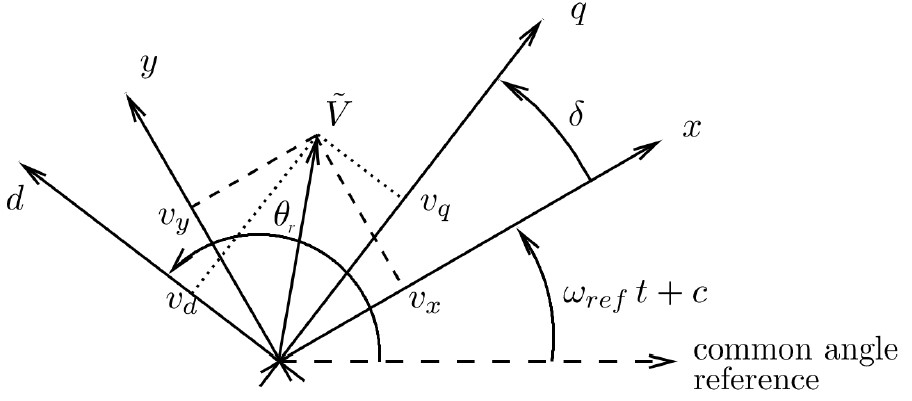
\includegraphics[width=109mm]{sync-delta.jpg}
\caption{Definition of the rotor angle $\delta$}\label{fig-sync-delta}
\end{figure}

The $d$ and $q$ components of the stator voltage relate to their $x$ and $y$ components through:
\begin{equation}\label{park-volt}
\left( \begin{array}{c} v_d \\ v_q \end{array} \right) = \left( \begin{array}{cc} - \sin \delta & \cos \delta \\ \cos \delta & \sin \delta \end{array} \right) \left( \begin{array}{c} v_x \\ v_y \end{array} \right)
\end{equation}
and similarly for the current:
\begin{equation}\label{park-cur}
\left( \begin{array}{c} i_d \\ i_q \end{array} \right) = \left( \begin{array}{cc} - \sin \delta & \cos \delta \\ \cos \delta & \sin \delta \end{array} \right) \left( \begin{array}{c} i_x \\ i_y \end{array} \right)
\end{equation}
where $\delta$ is the rotor angle.

Replacing $i_d$ and $i_q$ with the above expressions in Eqs.~(\ref{psiad-alg}, \ref{psiaq-alg}) gives:
\begin{equation}\label{psiad-alg-xy}
\psi_{ad} \left( \frac{1 + m ( \sqrt{\psi_{ad}^2 + \psi_{aq}^2} )^n}{M_d^u} + \frac{1}{L_{\ell f}} + \frac{S_{d1}}{L_{\ell d1}} \right) + \sin \delta \: i_x - \cos \delta \: i_y - \frac{1}{L_{\ell f}} \psi_f - \frac{S_{d1}}{L_{\ell d1}} \psi_{d1} = 0
\end{equation}
and similarly for the $q$ axis:
\begin{equation}\label{psiaq-alg-xy}
\psi_{aq} \left( \frac{1 + m ( \sqrt{\psi_{ad}^2 + \psi_{aq}^2} )^n}{M_q^u} + \frac{S_{q1}}{L_{\ell q1}} + \frac{S_{q2}}{L_{\ell q2}} \right) - \cos \delta \: i_x - \sin \delta \: i_y - \frac{S_{q1}}{L_{\ell q1}} \psi_{q1} - \frac{S_{q2}}{L_{\ell q2}} \psi_{q2} = 0
\end{equation}

\subsection{Park equations}

The original Park equations are written as:
\begin{eqnarray}
v_d & = & - R_a i_d - \omega \psi_q \label{park-vd} \\
v_q & = & - R_a i_q + \omega \psi_d \label{park-vq} \\
\frac{d\psi_f}{dt} & = & \omega_N ( K_f v_f - R_f i_f ) \label{park-psif} \\
\frac{d\psi_{d1}}{dt} & = & - \omega_N R_{d1} i_{d1} \label{park-psid1} \\
\frac{d\psi_{q1}}{dt} & = & - \omega_N R_{q1} i_{q1} \label{park-psiq1} \\
\frac{d\psi_{q2}}{dt} & = & - \omega_N R_{q2} i_{q2} \label{park-psiq2}
\end{eqnarray}
where $R_a$ is the stator resistance, $R_f$ the field winding resistance, $R_{d1}$, $R_{q1}$, $R_{q2}$ the rotor winding resistances, $\omega$ the rotor speed, $\omega_N$ the nominal angular frequency (in rad/s), $v_f$ the field voltage, and $K_f$ a coefficient to pass from per unit values of the excitation system to per unit values of the machine.

The stator equations are transformed as follows. Eqs.~(\ref{park-cur}) are used to express $v_d$, $v_q$, $i_d$ and $i_q$ as functions of $v_x$, $v_y$, $i_x$, $i_y$, while Eqs.~(\ref{psid-airgap}, \ref{psiq-airgap}) are used to involve $\psi_{ad}$ and $\psi_{aq}$. This yields for the $d$ axis:
\begin{eqnarray*}
v_d & = & - R_a ( - \sin \delta \: i_x + \cos \delta \: i_y ) - \omega ( L_\ell i_q + \psi_{aq} ) \\
    & = & - R_a ( - \sin \delta \: i_x + \cos \delta \: i_y ) - \omega L_\ell ( \cos \delta \: i_x + \sin \delta \: i_y ) - \omega \psi_{aq}
\end{eqnarray*}
and finally:
\begin{equation}\label{stator-d-xy}
0 = v_x \sin \delta - v_y \cos \delta + ( R_a \sin \delta - \omega L_\ell \cos \delta ) i_x - ( R_a \cos \delta + \omega L_\ell \sin \delta ) i_y - \omega \psi_{aq}
\end{equation}

The corresponding expressions in the $q$ axis are:
\begin{eqnarray}
v_q & = & - R_a ( \cos \delta \: i_x + \sin \delta \: i_y ) + \omega ( L_\ell i_d + \psi_{ad} ) \nonumber \\
    & = & - R_a ( \cos \delta \: i_x + \sin \delta \: i_y ) + \omega L_\ell ( - \sin \delta \: i_x + \cos \delta \: i_y ) + \omega \psi_{ad} \label{vq-xy}
\end{eqnarray}
and:
\begin{equation}\label{stator-q-xy}
0 = - \cos \delta v_x - \sin \delta v_y - ( R_a \cos \delta + \omega L_\ell \sin \delta ) i_x - ( R_a \sin \delta - \omega L_\ell \cos \delta ) i_y + \omega \psi_{ad}
\end{equation}

The rotor equations are transformed by substituting the expressions (\ref{if-rotor}, \ref{id1-rotor}, \ref{iq1-rotor}, \ref{iq2-rotor}) for the rotor currents, thereby obtaining:
\begin{eqnarray}
\frac{d\psi_f}{dt} & = & \omega_N ( K_f v_f - R_f \: \frac{\psi_f - \psi_{ad}}{L_{\ell f}} ) \label{rotor-psif} \\
\frac{d\psi_{d1}}{dt} & = & - \omega_N R_{d1} \: \frac{\psi_{d1} - S_{d1} \psi_{ad}}{L_{\ell d1}} \label{rotor-psid1} \\
\frac{d\psi_{q1}}{dt} & = & - \omega_N R_{q1} \: \frac{\psi_{q1} - S_{q1} \psi_{aq}}{L_{\ell q1}} \label{rotor-psiq1} \\
\frac{d\psi_{q2}}{dt} & = & - \omega_N R_{q2} \: \frac{\psi_{q2} - S_{q2} \psi_{aq}}{L_{\ell q2}} \label{rotor-psiq2}
\end{eqnarray}

\subsection{Rotor motion}

The equations of the rotor motion are:
\begin{eqnarray}
\frac{1}{\omega_N} \frac{d\delta}{dt} & = & \omega - \omega_{ref} \label{rotmot1} \\
2 H \frac{d\omega}{dt} & = & K_m T_m - T_e - D ( \omega - \omega_{ref} ) \label{rotmot2}
\end{eqnarray}
where $H$ is the inertia constant (in s), $\omega_{ref}$ the angular speed of the reference axes, $T_e$ is the electromagnetic torque, $T_m$ is the mechanical torque produced by the turbine and $K_m$ a coefficient to pass from per unit values of the turbine to per unit values of the machine.

The expression of $T_e$ is obtained as follows:
\begin{eqnarray}
T_e & = & \psi_d i_q - \psi_q i_d = ( L_\ell i_d + \psi_{ad} ) i_q - ( L_\ell i_q + \psi_{aq} ) i_d \nonumber \\
& = & \psi_{ad} i_q - \psi_{aq} i_d = \psi_{ad} ( \cos \delta \: i_x + \sin \delta \: i_y ) - \psi_{aq} ( - \sin \delta \: i_x + \cos \delta \: i_y ) \label{torque}
\end{eqnarray}

\subsection{Summing up: unknowns vs. equations}

The synchronous machine model involves 10 state variables, namely:
\begin{itemize}
\item 6 differential states: $\psi_f$, $\psi_{d1}$, $\psi_{q1}$, $\psi_{q2}$, $\delta$, $\omega$
\item 4 algebraic states: $i_x$, $i_y$, $\psi_{ad}$, $\psi_{aq}$.
\end{itemize}

They are balanced by:
\begin{itemize}
\item 4 algebraic equations: (\ref{psiad-alg-xy}, \ref{psiaq-alg-xy}, \ref{stator-d-xy}, \ref{stator-q-xy})
\item 6 differential equations: (\ref{rotor-psif}, \ref{rotor-psid1}, \ref{rotor-psiq1}, \ref{rotor-psiq2}, \ref{rotmot1}, \ref{rotmot2})
\end{itemize}

Well done!

\subsection{Per unit systems}

The above model relies on the EMFL per unit system, which allows writing the inductance matrices in the form shown in Eqs.~(\ref{sync-flux-d}, \ref{sync-flux-q}). On the other hand, it is more practical to have the excitation system and the turbine modelled in their own per unit systems. A change of base is thus necessary to interface those models.

\subsubsection*{Turbine}

The parameters of the turbine are expressed in per unit on the turbine nominal power $P_{nom}$ base (in MW), while those of the synchronous machine refer to the machine nominal apparent power $S_{nom}$ (in MVA). Both $P_{nom}$ and $S_{nom}$ are specified in the machine model (see Section~\ref{format-sync}).

\subsubsection*{Excitation system}

The case of the excitation system is a little more involved and requires specifying an additional parameter.

Let the base current of the field winding be $I_{fB}^{mac}$ in the machine model and $I_{fB}^{exc}$ in the excitation system model. Define the ratio:
\begin{equation}\label{ibratio-def}
{\cal R} = \frac{I_{fB}^{mac}}{I_{fB}^{exc}}.
\end{equation}

A given field current $i_f$ (in A) has the following value in per unit on the machine base :
\begin{equation}\label{ifpu-mac}
i_{f\,pu}^{mac} = \frac{i_f}{I_{fB}^{mac}}
\end{equation}
and the following value in per unit on the excitation system base :
\begin{equation}\label{ifpu-exc}
i_{f\,pu}^{exc} = \frac{i_f}{I_{fB}^{exc}}
\end{equation}
By combining Eqs.~(\ref{ibratio-def}, \ref{ifpu-mac}, \ref{ifpu-exc}):
\begin{equation}\label{ibratio-pu}
{\cal R} = \frac{i_{f\,pu}^{exc}}{i_{f\,pu}^{mac}}.
\end{equation}

The following are possible choices of per unit systems:

\begin{enumerate}
\item {\em Open-circuit unsaturated machine}

In this most often used per unit system, $I_{fB}^{exc}$ is the field current which produces the nominal stator voltage ($V = 1$ pu) when the machine rotates at its nominal speed ($\omega = 1$ pu) with its stator open ($i_d = i_q = 0$), saturation being neglected.

In these conditions, the machine Park equations give:
\[ v_d = \psi_q = \psi_{aq} = 0 \;\;\;\;\;\; v_q = \psi_d = \psi_{ad} = M_d^u \; i_{f\,pu}^{mac}. \]
Since:
\[ V = \sqrt{v_d^2 + v_q^2} = 1 \]
one has:
\[ M_d^u \; i_{f\,pu}^{mac} = 1 \]
while, on the excitation system base:
\[ i_{f\,pu}^{exc} = 1 \]
Introducing the last two relations in (\ref{ibratio-pu}) yields :
\begin{equation}\label{ibratio-unsat}
{\cal R} = M_d^u = X_d - X_\ell
\end{equation}
where $X_d$ is the unsaturated direct-axis synchronous reactance and $X_\ell$ the stator leakage reactance\footnote{in per unit $X_d^u = M_d^u$ and $X_\ell = L_\ell$}.

\item {\em Open-circuit saturated machine}

In this per unit system, $I_{fB}^{exc}$ is the field current which produces the nominal stator voltage ($V = 1$ pu) when the machine rotates at its nominal speed ($\omega = 1$ pu) with its stator open ($i_d = i_q = 0$), saturation being taken into account.

In these conditions, the machine Park equations give:
\[ v_d = \psi_q = \psi_{aq} = 0 \;\;\;\;\;\; v_q = \psi_d = \psi_{ad} = M_d \; i_{f\,pu}^{mac} \]
Since:
\[ V = \sqrt{v_d^2 + v_q^2} = 1 \]
one has:
\[ M_d \; i_{f\,pu}^{mac} = 1 \]
$M_d$ can be obtained from the saturation equation (\ref{md-sat}):
\[ M_d = \frac{M_d^u}{1 + m \: \psi_{ad}^n} = \frac{M_d^u}{1 + m \: ( M_d \; i_{f\,pu}^{mac} )^n} = \frac{M_d^u}{1+m} \]
while, on the excitation system base:
\[ i_{f\,pu}^{exc} = 1 \]
Introducing the last three relations in (\ref{ibratio-pu}) yields :
\begin{equation}\label{ibratio-sat}
{\cal R} = \frac{M_d^u}{1+m} = \frac{X_d - X_\ell}{1+m}
\end{equation}

\item {\em Saturated machine at nominal operating conditions}

In this per unit system, $I_{fB}^{exc}$ is the field current when the machine, rotating at its nominal speed ($\omega = 1$ pu), produces its nominal active and reactive powers under its nominal stator voltage ($V = 1$ pu, $P = \cos \phi_N$ and $Q = \sin \phi_N$), saturation being taken into account.
\end{enumerate}

\subsection{\index{SYNCMACH@SYNC\_MACH}Data format}\label{format-sync}

Synchronous machines are specified by SYNC\_MACH records. There are two variants, depending on the value of the {\tt MOD\_TYPE} field:
\begin{itemize}
\item if {\tt MOD\_TYPE} is set to the (string value) {\tt XT}, the data relate to reactances and time constants that are used internally to determine the resistances and inductances involved in Eqs.~(\ref{sync-flux-d}, \ref{sync-flux-q}, \ref{park-vd}-\ref{park-psiq2})
\item if {\tt MOD\_TYPE} is set to {\tt RL}, the data relate to those resistances and inductances directly.
\end{itemize}

The two sets of data are described next.

\subsubsection*{First variant: reactances and time constants are specified}

The data format is as follows.

\hspace*{5ex}{\tt SYNC\_MACH NAME BUS FP FQ P Q SNOM PNOM H D IBRATIO} \\
\hspace*{10ex}{\tt MOD\_TYPE XL XD XPD XSD XQ XPQ XSQ M N RA TPD0 TSD0 TPQ0 TSQ0} \\
\hspace*{10ex}{\bf EXC} {\tt E1 E2 ...\ EN} \; {\bf TOR} {\tt T1 T2 ...\ TN ;}

where:
\begin{itemize}
\item {\tt NAME} is the name of the machine. This is a string of at most 20 characters
\item {\tt BUS} is the name of the bus which the machine is connected to. This is a string of at most 8 characters
\item {\tt FP} is the fraction $f_P$ of the initial bus active power injection, as defined in Eq.~(\ref{frac}) (see Section~\ref{sec-refframe})
\item {\tt FQ} is the fraction $f_Q$ of the initial bus reactive power injection, as defined in Eq.~(\ref{frac})
\item {\tt P} is the initial active power injected by the machine, in MW, denoted by $P^c_j$ in Eq.~(\ref{inipower}) (see Section~\ref{sec-refframe})
\item {\tt Q} is the initial reactive power injected by the machine, in Mvar, denoted by $Q^c_j$ in Eq.~(\ref{inipower})
\item {\tt SNOM} is the nominal apparent power of the machine, in MVA. It is used as base power in the machine model
\item {\tt PNOM} is the nominal active power of the machine, in MW. It is used as base power for the turbine model
\item {\tt H} is the inertia time constant $H$ in Eq.~(\ref{rotmot2}), in s
\item {\tt D} is the damping time constant $D$ in Eq.~(\ref{rotmot2}), in pu. $D$ is usually set to zero when the damper windings are modelled
\item {\tt IBRATIO} is the dimensionless current ratio ${\cal R}$ as defined in Eq.~(\ref{ibratio-pu})
\item {\tt MOD\_TYPE} is set to the string `XT' in this variant (the quotes are not needed)
\item {\tt XL} is the armature leakage reactance, in pu
\item {\tt XD} is the unsaturated direct-axis synchronous reactance, in pu
\item {\tt XPD} is the direct-axis transient reactance, in pu
\item {\tt XSD} is the direct-axis subtransient reactance, in pu
\item {\tt XQ} is the unsaturated quadrature-axis synchronous reactance, in pu
\item {\tt XPQ} is the quadrature-axis transient reactance, in pu
\item {\tt XSQ} is the quadrature-axis subtransient reactance, in pu
\item {\tt M} is the dimensionless saturation factor $m$ as defined in Eqs.~(\ref{md-sat}, \ref{mq-sat}). {\tt M} is set to zero if saturation is neglected
\item {\tt N} is the dimensionless saturation exponent $n$ as defined in Eqs.~(\ref{md-sat}, \ref{mq-sat}). The value is ignored if {\tt M} is set to zero
\item {\tt RA} is the armature resistance, in pu
\item {\tt TPD0} is the direct-axis open-circuit transient time constant, in s. It is usually denoted $T'_{d0}$
\item {\tt TSD0} is the direct-axis open-circuit subtransient time constant, in s. It is usually denoted $T''_{d0}$
\item {\tt TPQ0} is the quadrature-axis open-circuit transient time constant, in s. It is usually denoted $T'_{q0}$
\item {\tt TSQ0} is the quadrature-axis open-circuit subtransient time constant, in s. It is usually denoted $T''_{q0}$
\item {\bf EXC} is a keyword (not a data !) indicating the beginning of the excitation system data section
\item {\tt E1 E2 ...\ EN} are the successive excitation system data. Please refer to Section~\ref{sec-model-data} for more details
\item {\bf TOR} is a keyword (not a data !) indicating the end of the excitation system data and the beginning of the torque control data section
\item {\tt T1 T2 ...\ TN} are the successive torque control data. Please refer to Section~\ref{sec-model-data} for more details
\end{itemize}

\subsubsection*{Second variant: resistances and inductances are specified}

The data format is as follows.

\hspace*{5ex}{\tt SYNC\_MACH NAME BUS FP FQ P Q SNOM PNOM H D IBRATIO} \\
\hspace*{10ex}{\tt MOD\_TYPE LL MDU LLF LLD1 MQU LLQ1 LLQ2 M N RA RF RD1 RQ1 RQ2} \\
\hspace*{10ex}{\bf EXC} {\tt E1 E2 ...\ EN} \; {\bf TOR} {\tt T1 T2 ...\ TN ;}

where:
\begin{itemize}
\item {\tt NAME} is the name of the machine. This is a string of at most 20 characters
\item {\tt BUS} is the name of the bus which the machine is connected to. This is a string of at most 8 characters
\item {\tt FP} is the fraction $f_P$ of the initial bus active power injection, as defined in Eq.~(\ref{frac}) (see Section~\ref{sec-refframe})
\item {\tt FQ} is the fraction $f_Q$ of the initial bus reactive power injection, as defined in Eq.~(\ref{frac})
\item {\tt P} is the initial active power injected by the machine, in MW, denoted by $P^c_j$ in Eq.~(\ref{inipower}) (see Section~\ref{sec-refframe})
\item {\tt Q} is the initial reactive power injected by the machine, in Mvar, denoted by $Q^c_j$ in Eq.~(\ref{inipower})
\item {\tt SNOM} is the nominal apparent power of the machine, in MVA. It is used as base power in the machine model
\item {\tt PNOM} is the nominal active power of the machine, in MW. It is used as base power for the turbine model
\item {\tt H} is the inertia time constant $H$ in Eq.~(\ref{rotmot2}), in s
\item {\tt D} is the damping time constant $D$ in Eq.~(\ref{rotmot2}), in pu. $D$ is usually set to zero when the damper windings are modelled
\item {\tt IBRATIO} is the dimensionless current ratio ${\cal R}$ as defined in Eq.~(\ref{ibratio-pu})
\item {\tt MOD\_TYPE} is set to the string `RL' in this variant (the quotes are not needed)
\item {\tt LL} is the leakage inductance $L_\ell$ of the armature, in pu
\item {\tt MDU} is the direct-axis unsaturated mutual inductance $M_d$, in pu
\item {\tt LLF} is the leakage inductance $L_{\ell f}$ of the field winding, in pu
\item {\tt LLD1} is the leakage inductance $L_{\ell d1}$ of the $d1$ damper winding, in pu
\item {\tt MQU} is the quadrature-axis unsaturated mutual inductance $M_q$, in pu
\item {\tt LLQ1} is the leakage inductance $L_{\ell q1}$ of the $q1$ damper winding, in pu
\item {\tt LLQ2} is the leakage inductance $L_{\ell q2}$ of the $q2$ damper winding, in pu
\item {\tt M} is the dimensionless saturation factor $m$ as defined in Eqs.~(\ref{md-sat}, \ref{mq-sat}). {\tt M} is set to zero if saturation is neglected
\item {\tt N} is the dimensionless saturation exponent $n$ as defined in Eqs.~(\ref{md-sat}, \ref{mq-sat}). The value is ignored if {\tt M} is set to zero
\item {\tt RA} is the armature resistance, in pu
\item {\tt RF} is the resistance $R_f$ of the field winding, in pu
\item {\tt RD1} is the resistance $R_{d1}$ of the $d1$ damper winding, in pu
\item {\tt RQ1} is the resistance $R_{q1}$ of the $q1$ damper winding, in pu
\item {\tt RQ2} is the resistance $R_{q2}$ of the $q2$ damper winding, in pu
\item {\bf EXC} is a keyword (not a data !) indicating the beginning of the excitation system data section
\item {\tt E1 E2 ...\ EN} are the successive excitation system data. Please refer to Section~\ref{sec-model-data} for more details
\item {\bf TOR} is a keyword (not a data !) indicating the end of the excitation system data and the beginning of the torque control data section
\item {\tt T1 T2 ...\ TN} are the successive torque control data. Please refer to Section~\ref{sec-model-data} for more details.
\end{itemize}

As explained in the preamble of this section, the full model can be simplified by ignoring some of the rotor windings\footnote{let us recall that not all combinations of windings are allowed}. This is specified by replacing the values of some parameters with an asterisk `*' (the quotes are not needed). The parameters of concern are detailed in Table~\ref{tab-sync-simplified}.

\begin{table}[htb]
\centering
\caption{Simplified model specification (the quotes are not needed)}\label{tab-sync-simplified}
{\footnotesize
\begin{tabular}{|c|c|c|}
\hline
simplification & {\tt MOD\_TYPE} = `XT' & {\tt MOD\_TYPE} = `RL' \\ \hline
no $d1$ winding ($S_{d1} = 0$) & replace values of {\tt XSD} and {\tt TSD0} by `*' & replace values of {\tt LLD1} and {\tt RD1} by `*' \\
no $q1$ winding ($S_{q1} = 0$) & replace values of {\tt XPQ} and {\tt TPQ0} by `*' & replace values of {\tt LLQ1} and {\tt RQ1} by `*' \\
no $q2$ winding ($S_{q2} = 0$) & replace values of {\tt XSQ} and {\tt TSQ0} by `*' & replace values of {\tt LLQ2} and {\tt RQ2} by `*' \\ \hline
\end{tabular}
}
\end{table}

\subsection{Initialization}

\begin{quote}
\faHandPointRight ~ Here is an example of output produced by RAMSES at initialization.
\end{quote}
{\scriptsize
\begin{verbatim}
NUMBER OF ISLANDS :    1

     5 buses in island #     1 (includes a Thevenin equivalent)

NUMBER OF SHUNTS :     0  (B_ type:     0)

NUMBER OF SYNCHRONOUS MACHINES :    1

machine              at bus                 V            P           Q        delta    sat    island  br
                     excit model          vf(pu)   torque model               Tm(pu)

G5                   5                    1.0000    450.00186     68.49769    70.99   1.0000       1    1
                     exc_GENERIC3         2.3680   THERMAL_GENERIC1          0.97826
\end{verbatim}
}
\begin{quote}
In this example, the model involves a single synchronous machine, named G5, connected to bus 5. The network is connected (single island, numbered 1). The machine is in service ({\tt br = 1}) and injects around 450 MW and 68 Mvar into the grid, under a bus voltage of 1 pu.

{\tt delta} is the initial value of the rotor angle $\delta$, in degrees; see Fig.~\ref{fig-sync-delta}.

{\tt sat} is the saturation factor defined by:
\begin{equation}\label{sat-factor}
sat = 1 + m \left( \sqrt{\psi_{ad}^2 + \psi_{aq}^2} \right)^n \geq 1
\end{equation}
This is the ratio between the field current in the saturated machine and the corresponding field current when saturation is neglected, for the same operating conditions. Thus, it characterizes the extra excitation current needed in the presence of saturated material. In the above example, saturation was neglected (a zero value was specified for {\tt M}) and, hence, $sat = 1$.

The machine has an excitation controller whose model is named {\tt exc\_GENERIC3}. At the initial operating point the field voltage is $v_f = 2.3680$ pu on the exciter base, which is indirectly defined by the {\tt IBRATIO} parameter of the machine.

The machine is driven by a turbine whose model is named {\tt THERMAL\_GENERIC1}. The initial mechanical torque is $T_m = 0.97826$ pu, on the turbine base, which is defined by the {\tt PNOM} parameter of the machine.
\end{quote}

%------------------------------------------------------------------------------------------
\section{\index{THEVEQ}\index{Infinite Bus}Th\'{e}venin equivalents}

\subsection{Modelling}

Th\'{e}venin equivalents are used to represent ``external'' systems in a simplified manner.

The equivalent includes a voltage source $\bar{E}_{th}$ in series with a reactance $X_{th}$, as shown in Fig.~\ref{fig-thevenin}. The voltage source has a constant frequency, equal to the nominal value given by the FNOM record. It has constant magnitude and phase angle. The latter are determined at initialisation from the bus voltage and the injected powers.

\begin{figure}[htb]
\centering
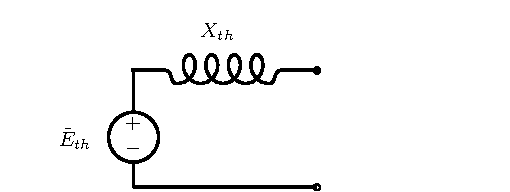
\includegraphics[scale=1.0]{thevenin.pdf}
\caption{Th\'{e}venin equivalent}\label{fig-thevenin}
\end{figure}

The Th\'{e}venin reactance is specified through the {\em short-circuit power}\footnote{also known as fault level}:
\begin{equation}\label{ssc-def}
S_{sc\;MVA} = \frac{U_{nom}^2}{X_{th\;\Omega}}
\end{equation}
where $U_{nom}$ is the nominal voltage (in kV) of the bus to which the Th\'{e}venin equivalent is connected, and $X_{th\;\Omega}$ is the Th\'{e}venin reactance in Ohm.

Note that $S_{sc\;MVA}$ is the short-circuit of the Th\'{e}venin equivalent {\em alone}; it is not the short-circuit at the bus where the equivalent is connected, which depends on the other components present in the system.

Taking $U_{nom}$ as base voltage and $S_B$ as base power, the Th\'{e}venin reactance in per unit is given by:
\begin{equation}\label{xth-pu}
X_{th\;pu} = \frac{X_{th\;\Omega}}{Z_B} = \frac{X_{th\;\Omega} \; S_B}{U_{nom}^2} = \frac{S_B}{S_{sc\;MVA}} = \frac{1}{S_{sc\;pu}}
\end{equation}
where $Z_B$ is the base impedance and $S_{sc\;pu}$ the short-circuit power in per unit.

\subsection{Data format}\label{format-thev}

Th\'{e}venin equivalents are specified as injectors with model name THEVEQ. The format is as follows:

\hspace*{5ex}{\tt INJEC THEVEQ NAME BUS FP FQ P Q SSC ;}

where:
\begin{itemize}
\item {\tt NAME} is the name of the Th\'{e}venin equivalent. This is a string of at most 20 characters
\item {\tt BUS} is the name of the bus which the equivalent is connected to. This is a string of at most 8 characters
\item {\tt FP} is the fraction $f_P$ of the initial bus active power injection, as defined in Eq.~(\ref{frac}) (see Section~\ref{sec-refframe})
\item {\tt FQ} is the fraction $f_Q$ of the initial bus reactive power injection, as defined in Eq.~(\ref{frac})
\item {\tt P} is the initial active power injected by the machine, in MW, denoted by $P^c_j$ in Eq.~(\ref{inipower}) (see Section~\ref{sec-refframe})
\item {\tt Q} is the initial reactive power injected by the machine, in Mvar, denoted by $Q^c_j$ in Eq.~(\ref{inipower})
\item {\tt SSC} is the short-circuit power, in MVA, as defined in Eq.~(\ref{ssc-def}).
\end{itemize}

%------------------------------------------------------------------------------------------
\section{\index{IMPLOAD}Impedance loads}

\subsection{Modelling}

An impedance load\footnote{to be more precise: a constant impedance load. The formulation in terms of admittance is preferred here} is merely modelled by a shunt admittance. The active power $P$ (resp. reactive power $Q$) consumed varies with the square of the bus voltage magnitude $V$ according to:
\begin{equation}\label{impload-pq}
P = G \; V^2 \;\;\;\;\;\; Q = - B \; V^2
\end{equation}
where $G$ (resp. $B$) is the shunt conductance (resp. susceptance). Both are determined at initialization and remain constant (unless they are changed by a user-defined action). Let us recall that $B$ is negative (resp. positive) for an inductive (resp. capacitive) load.

\subsection{Data format}\label{format-impload}

Impedance loads are specified by IMPLOAD records. The format is as follows:

\hspace*{5ex}{\tt IMPLOAD NAME BUS FP FQ P Q ;}

where:
\begin{itemize}
\item {\tt NAME} is the name of the load. This is a string of at most 20 characters. It must not start with `M\_': this prefix is reserved to denote a mismatch load (see Section~\ref{sec-ini-proc})
\item {\tt BUS} is the name of the bus which the load is connected to. This is a string of at most 8 characters
\item {\tt FP} is the fraction $f_P$ of the initial bus active power injection, as defined in Eq.~(\ref{frac}) (see Section~\ref{sec-refframe})
\item {\tt FQ} is the fraction $f_Q$ of the initial bus reactive power injection, as defined in Eq.~(\ref{frac})
\item {\tt P} is the initial active power injected by the machine, in MW, denoted by $P^c_j$ in Eq.~(\ref{inipower}) (see Section~\ref{sec-refframe})
\item {\tt Q} is the initial reactive power injected by the machine, in Mvar, denoted by $Q^c_j$ in Eq.~(\ref{inipower}).
\end{itemize}
